\chapter{Manuel d’utilisation}

\section{Compilation du programme}

Afin de compiler l'application, suivez ces différentes étapes :
\begin{itemize}
	\item assurez-vous de disposer de GCC~;
	\item assurez-vous de disposer d'une version pour développeurs de GTK+ 2~;
	\item depuis un terminal, naviguez jusqu'au dossier des sources de Link-Pix~;
	\item lancez \verb|make|.
\end{itemize}

\section{Démarrage du programme}

Pour démarer Link-Pix il suffit d'exécuter le binaire \verb|link-pix| généré par \verb|make|, que ce soit en ligne de commande ou par votre gestionnaire de fichiers.

\begin{figure}[h!]
      \centering
      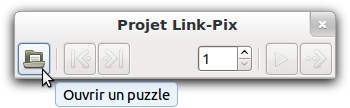
\includegraphics[scale=0.5]{gui-1}
      \caption{Link-Pix à son lancement.}
\end{figure}

\section{Ouverture d'un puzzle}

Pour ouvrir un puzzle il suffit de cliquer sur le bouton prévu à cet effet dans la fenêtre de Link-Pix.
Une boîte de dialogue apparaîtra alors, vous proposant de charger un fichier \verb|.lnpx| (voir \ref{chargement}). Quelques fichiers \verb|.lnpx| sont fournis avec les sources de l'application.

\begin{figure}[b!]
      \centering
      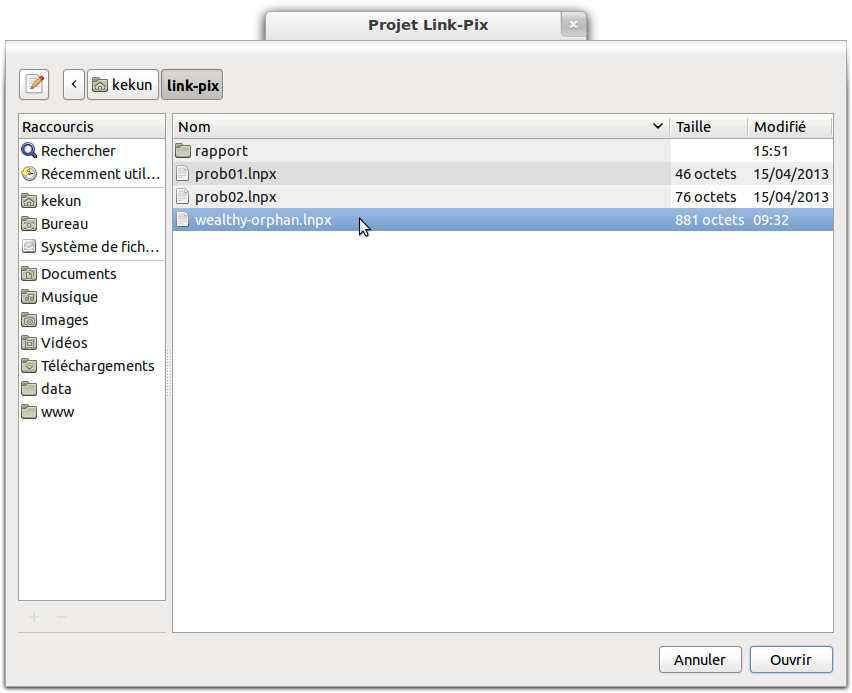
\includegraphics[scale=0.5]{gui-2}
      \caption{La boîte de dialogue d'ouverture de puzzle de Link-Pix.}
      \label{chargement}
\end{figure}

\section{Résolution du puzzle}

\subsection{Fonctionnalités de l'interface graphique}

\begin{figure}[h!]
      \centering
      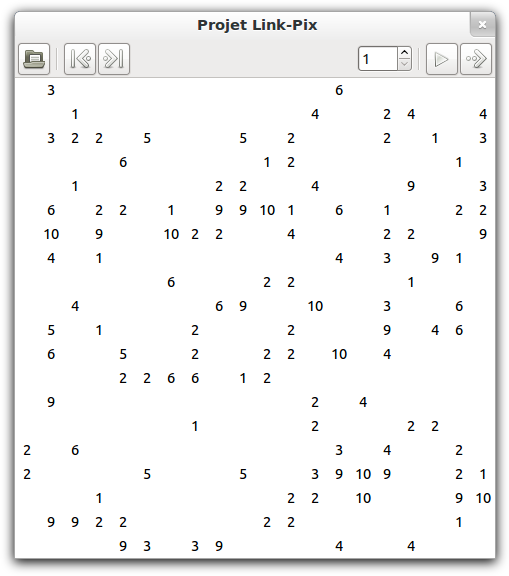
\includegraphics[scale=0.5]{gui-3}
      \caption{Link-Pix lorsqu'un puzzle est ouvert.}
\end{figure}

L'interface graphique vous permet :
\begin{itemize}
	\item d'ouvrir un fichier de puzzle~;
	\item de recharger le puzzle~;
	\item de résoudre le puzzle~;
	\item de définir le nombre d'étapes à résoudre à chaque pas, afin d'accélérer la résolution~;
	\item d'avancer pas à pas automatiquement dans la résolution du puzzle~;
	\item d'avancer pas à pas manuellement dans la résolution du puzzle~;
	\item d'afficher le puzzle tout au long de sa résolution avec des couleurs différentes indiquant son état.
\end{itemize}

\subsection{Légende des couleurs}

\begin{figure}[h!]
      \centering
      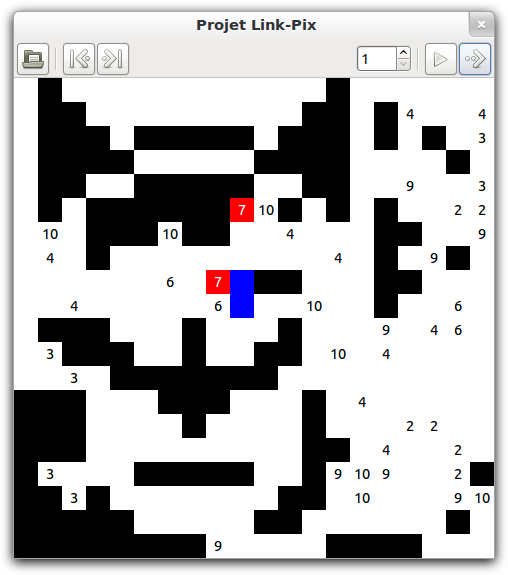
\includegraphics[scale=0.5]{gui-4}
      \caption{Link-Pix en cours de résolution d'un puzzle.}
\end{figure}

Lors de la résolution, chaque case peut apparaître d'une des manières suivantes :
\begin{itemize}
	\item une case blanche sans nombre est une case actuellement vide~;
	\item une case blanche avec nombre est une case encore non résolue~;
	\item une case noire est une case remplie lors de la résolution du puzzle~;
	\item une case bleue est une case remplie au cours de la dernière étape de résolution, elle deviendra noire au tour suivant~;
	\item une case rouge est une case appairée dont la résolution a avancé au cours du dernier tour de résolution mais pas encore totalement résolue, le nombre est la distance restant à parcourir jusqu'à son pair.
\end{itemize}

